\documentclass[aspectratio=169]{beamer}
\usepackage{will_handley_beamer}
\usepackage{title_page}
\usepackage{pythonhighlight}
\usepackage{tikz}
\newcommand{\av}[2][]{\left\langle #2\right\rangle_{#1}}

% Commands
% --------
% - \arxiv{arxiv number}
% - \cols{width}{lh column}{rh column}
% -  \begin{fig(left|right)}[fractional width (e.g 0.6) ]{name of image}
%        content of other column
%    \end{fig(left|right)}

% Talk details
% ------------
\title{ Nested sampling: {\large powering next-generation inference and machine learning tools}}
\subtitle{for cosmology, particle physics and beyond}
\date{18\textsuperscript{th} August 2023}

\begin{document}



\begin{frame}
    \titlepage
\end{frame}

\begin{frame}
    \frametitle{Highlight: state-of-the-art Nature review [\href{https://www.nature.com/articles/s43586-022-00121-x}{NatRev}]}
    \begin{columns}
        \column{0.5\textwidth}
        \begin{itemize}
            \item Invented by John Skilling in 2004.
            \item Recent Nature review primer on nested sampling led by Andrew Fowlie and assembled by the community.
            \item Showcases the current set of tools, and applications from chemistry to cosmology.
            \item Recent 1.5 day conference in Munich: ``Frontiers of Nested Sampling''
            \item Planned week-long NSCON 2024
            \item In this talk:
                \begin{itemize}
                    \item User guide to nested sampling
                    \item Particle physics applications
                    \item Cosmology applications
                    \item Machine learning applications
                \end{itemize}
        \end{itemize}
        \column{0.3\textwidth}
        \includegraphics[width=\textwidth]{figures/nature1}
        \includegraphics[width=\textwidth]{figures/nature2}
        \column{0.2\textwidth}
        \includegraphics[width=\textwidth]{figures/nature4}
        \includegraphics[width=\textwidth]{figures/nature5}
    \end{columns}

\end{frame}

\begin{frame}
    \frametitle{Where is Nested Sampling?}
    \begin{columns}
        \column{0.5\textwidth}
        \begin{itemize}
            \item For many purposes, in your Neural Net you should group Nested Sampling with (MCMC) techniques such as:
                \begin{itemize}
                    \item Metropolis-Hastings (PyMC, MontePython)
                    \item Hamiltonian Monte Carlo (Stan, blackjax)
                    \item Ensemble sampling (emcee, zeus). 
                    \item Variational Inference (Pyro)
                    \item Sequential Monte Carlo 
                    \item Thermodynamic integration
                    \item Genetic algorithms
                \end{itemize}
            \item You may have heard of it branded form:
                \begin{itemize}
                    \item MultiNest
                    \item PolyChord
                    \item dynesty
                    \item ultranest
                \end{itemize}
            \end{itemize}
        \column{0.5\textwidth}
        \begin{columns}
            \column{0.5\textwidth}
        \includegraphics[width=\textwidth]{figures/emcee}
        \includegraphics[width=\textwidth]{figures/metropolis-hastings}
            \column{0.5\textwidth}
        \includegraphics[width=\textwidth]{figures/zeus}
        \end{columns}
        \includegraphics[width=\textwidth]{figures/hmc_explained}
    \end{columns}
\end{frame}


\begin{frame}
    \frametitle{What is Nested Sampling?}
    \begin{itemize}
        \item Nested sampling is a radical, multi-purpose numerical tool.
        \item Given a (scalar) function $f$ with a vector of parameters $\theta$, it can be used for:
    \end{itemize}
    \vspace{-10pt}
    \begin{columns}[t]
        \column{0.3\textwidth}
        \begin{block}{Optimisation}
            \[\theta_\text{max} = \max_\theta{f(\theta)}\]
        \end{block}
        \column{0.3\textwidth}
        \begin{block}{Exploration}
            \vspace{-10pt}
            \[\text{draw/sample}\quad \theta\sim f\]
            \vspace{-15pt}
        \end{block}
        \column{0.3\textwidth}
        \begin{block}{Integration}
            \[\int f(\theta) dV \]
        \end{block}
    \end{columns}
    \begin{columns}[t]
        \column{0.33\textwidth}
        \centerline{\includegraphics[width=0.8\textwidth,page=13]{figures/himmelblau}}
        \column{0.33\textwidth}
        \centerline{\includegraphics[width=0.8\textwidth,page=15]{figures/himmelblau}}
        \column{0.33\textwidth}
        \centerline{\includegraphics[width=0.8\textwidth,page=14]{figures/himmelblau}}
    \end{columns}
\end{frame}

\begin{frame}
    \frametitle{The three pillars of Bayesian inference}
    \begin{columns}[t]
        \column{0.33\textwidth}
        \begin{block}{Parameter estimation}
            What do the data tell us about the parameters of a model?

            \textit{e.g. the size or age of a $\Lambda$CDM universe}
            \[ \hspace{-4pt}\C[0]{P(\theta|D,M)} = \frac{\C[2]{P(D|\theta,M)} \C[1]{P(\theta|M)}}{\C[3]{P(D|M)}} \] 
            \[ \C[0]{\mathcal{P}} = \frac{\C[2]{\mathcal{L}} \times\C[1]{\pi}}{\C[3]{\mathcal{Z}}}\] 
            \[ \C[0]{\text{Posterior}} = \frac{\C[2]{\text{Likelihood}} \times\C[1]{\text{Prior}}}{\C[3]{\text{Evidence}}}\]
        \end{block}
        \column{0.3\textwidth}
        \begin{block}{Model comparison}
            How much does the data support a particular model?

            \textit{e.g. $\Lambda$CDM vs a dynamic dark energy cosmology}
            \[ \C[4]{P(M|D)} = \frac{\C[3]{P(D|M)} \C[5]{P(M)}}{\C[7]{P(D)}} \vspace{-7pt}\]
            \[ \frac{\C[3]{\mathcal{Z}_\mathcal{M}} \C[5]{\Pi_\mathcal{M}}}{\C[7]{\sum_m Z_m \Pi_m}} \]
            \[ \C[4]{\text{Posterior}} = \frac{\C[3]{\text{Evidence}} \times\C[5]{\text{Prior}}}{\C[7]{\text{Normalisation}}}\]
        \end{block}
        \column{0.33\textwidth}
        \begin{block}{Tension quantification}
            Do different datasets make consistent predictions from the same model? 
            \textit{e.g. CMB vs Type IA supernovae data}
            \[ \mathcal{R} = \frac{\C[3]{\mathcal{Z}}_{AB}}{\C[3]{\mathcal{Z}}_A\C[3]{\mathcal{Z}}_\mathcal{B}}\] 
            \[
                \begin{aligned} \log\mathcal{S} = \av[{\C[0]{\mathcal{P}}_{AB}}]{\C[2]{\log\mathcal{L}}_{AB}}&\\
                    -\av[{\C[0]{\mathcal{P}}_{A}}]{\C[2]{\log\mathcal{L}}_{A}}&\\
                    -\av[{\C[0]{\mathcal{P}}_{B}}]{\C[2]{\log\mathcal{L}}_{B}}&
                \end{aligned}
            \]
        \end{block}
    \end{columns}
\end{frame}

\begin{frame}
    \frametitle{Why do sampling?}
    \begin{columns}
        \column{0.5\textwidth}
        \vspace{-10pt}
        \begin{itemize}
            \item The cornerstone of numerical Bayesian inference is working with \textbf{samples}.
            \item Generate a set of representative parameters drawn in proportion a distributionto the posterior $\theta\sim\C[0]{\mathcal{P}}$.
            \item The magic of marginalisation $\Rightarrow$ perform usual analysis on each sample in turn.
            \item The golden rule is \C[3]{stay in samples} until the last moment before computing summary statistics/triangle plots because \[\boxed{f(\:\av{X}\:)\ne \av{\:f(X)\:}}\]
            \item Generally need $\sim\mathcal{O}(12)$ independent samples to compute a value and error bar.
        \end{itemize}
        \column{0.5\textwidth}
        \includegraphics[width=\textwidth]{figures/samples.pdf}
    \end{columns}
\end{frame}

\begin{frame}
    \begin{columns}
        \column{0.48\textwidth}
        \begin{block}{\textbf{MCMC}}
            \only<16>{
                \begin{itemize}
                    \item Single ``walker''
                    \item Explores posterior
                    \item Fast, if proposal matrix is tuned
                    \item Parameter estimation, suspiciousness calculation
                    \item Channel capacity optimised for generating posterior samples
                \end{itemize}
            }
        \end{block}
            \includegraphics<1>[width=\textwidth,page=16]{figures/himmelblau}%
            \includegraphics<2>[width=\textwidth,page=17]{figures/himmelblau}%
            \includegraphics<3>[width=\textwidth,page=18]{figures/himmelblau}%
            \includegraphics<4>[width=\textwidth,page=19]{figures/himmelblau}%
            \includegraphics<5>[width=\textwidth,page=20]{figures/himmelblau}%
            \includegraphics<6-15>[width=\textwidth,page=21]{figures/himmelblau}%
        \centerline{\includegraphics<16>[width=0.5\textwidth,page=19]{figures/himmelblau}}
        \column{0.48\textwidth}
        \begin{block}<7->{\textbf{Nested sampling}}
            \only<16>{
                \begin{itemize}
                    \item Ensemble of ``live points''
                    \item Scans from prior to peak of likelihood
                    \item Slower, no tuning required
                    \item Parameter estimation, model comparison, tension quantification
                    \item Channel capacity optimised for computing partition function
                \end{itemize}
            }
        \end{block}
            \includegraphics<7|handout:0>[width=\textwidth,page=1]{figures/himmelblau}%
            \includegraphics<8|handout:0>[width=\textwidth,page=2]{figures/himmelblau}%
            \includegraphics<9|handout:0>[width=\textwidth,page=3]{figures/himmelblau}%
            \includegraphics<10          >[width=\textwidth,page=4]{figures/himmelblau}%
            \includegraphics<11|handout:0>[width=\textwidth,page=5]{figures/himmelblau}%
            \includegraphics<12|handout:0>[width=\textwidth,page=6]{figures/himmelblau}%
            \includegraphics<13|handout:0>[width=\textwidth,page=7]{figures/himmelblau}%
            \includegraphics<14|handout:0>[width=\textwidth,page=8]{figures/himmelblau}%
            \includegraphics<15|handout:0>[width=\textwidth,page=15]{figures/himmelblau}%
        \centerline{\includegraphics<16>[width=0.5\textwidth,page=4]{figures/himmelblau}} 
    \end{columns}
\end{frame}

\begin{frame}
    \frametitle{Nested sampling}
    \begin{columns}
        \column{0.6\textwidth}
        \begin{itemize}
            \item Sequentially update a set $S$ of $n$ samples:
                \begin{itemize}
                    \item[$S_0$:]  Generate $n$ samples uniformly over the space (from the prior $\pi$). 

                    \item[$S_{i+1}$:] Delete the lowest likelihood sample in $S_{i}$, and replace it with a new uniform sample with higher likelihood.
                \end{itemize}
            \item Requires one to be able to sample uniformly within a region, subject to a {\em hard likelihood constraint}:
                \[\{\theta\sim \pi : \mathcal{L}(\theta)>\mathcal{L}_*. \}\]
            \item This procedure optimises (multimodally), and can calculate the \C[3]{evidence} \& \C[0]{posterior} weights.
            \item The evolving ensemble of live points allows algorithms to perform self-tuning and mode clustering.
        \end{itemize}
        \column{0.4\textwidth}
        \includegraphics[width=\textwidth,page=4]{figures/himmelblau}%
    \end{columns}
\end{frame}

\begin{frame}
    \frametitle{Integration in Physics}
    \begin{itemize}
        \item Integration is a fundamental concept in physics, statistics and data science:
    \end{itemize}
    \begin{columns}
        \column{0.3\textwidth}
        \begin{block}{Partition functions}
            \vspace{-11pt}
            \[ Z(\beta) = \int e^{-\beta H(q,p)} dq dp \]
        \end{block}
        \column{0.3\textwidth}
        \begin{block}{Path integrals}
            \[ \Psi = \int e^{i S} \mathcal{D}x \]
        \end{block}
        \column{0.3\textwidth}
        \begin{block}{Bayesian marginals}
            \vspace{-11pt}
            \[ \mathcal{Z}(D) = \int \mathcal{L}(D|\theta) \pi(\theta) d\theta \]
        \end{block}
    \end{columns}
    \begin{columns}
        \column{0.6\textwidth}
        \begin{itemize}
            \item Need numerical tools if analytic solution unavailable.
            \item High-dimensional numerical integration is hard.
            \item Riemannian strategy estimates volumes geometrically:
                \[ \int f(x) d^nx \approx \sum_i f(x_i) \Delta V_i \sim \mathcal{O}(e^n) \]
            \item Curse of dimensionality $\Rightarrow$ exponential scaling.
            \item Nested sampling integrates \textbf{probabilistically}.
        \end{itemize}
        \column{0.4\textwidth}
        \includegraphics[width=\textwidth]{figures/integration.pdf}
    \end{columns}
\end{frame}

\begin{frame}
    \frametitle{Integration in high dimensions}
    \begin{columns}
        \column{0.6\textwidth}
        \begin{itemize}
            \item Nested sampling can compute the \C[3]{Bayesian evidence} $\C[3]{\mathcal{Z}} = \int\C[2]{\mathcal{L}(\theta)}\C[1]{\pi(\theta)}d\theta$
            \item Numerical integration $\int f(x) dV$ in high dimensions is hard.
            \item \texttt{scipy.integrate(...)} is unusable in more than four dimensions.
            \item This is due to the curse of dimensionality: need to sum $\sim N^d$ units to compute $\approx \sum_i f(x_i) \Delta V_i$.
            \item Additionally, estimating volumes with geometry becomes exponentially hard as $d$ increases.
            \item \textit{Aside: \textbf{Riemannian integration} (blue) is taught as standard. An orthogonal approach (red) [usually theoretical] is \textbf{Lesbesgue integration}.}
        \end{itemize}
        \column{0.4\textwidth}
        \includegraphics[width=\textwidth]{figures/integration}
        \includegraphics[width=\textwidth]{figures/2560px-Riemannvslebesgue.svg.png}
    \end{columns}
\end{frame}

\begin{frame}
    \frametitle{Probabalistic volume estimation}
    \begin{columns}
        \column{0.5\textwidth}
        \begin{itemize}
            \item Key idea in NS: estimating volumes probabilistically
        \[
            \frac{\C[1]{V_\mathrm{after}}}{\C[0]{V_\mathrm{before}}} 
            \approx \frac{\C[1]{n_\mathrm{in}}}{\C[0]{n_\mathrm{out}}+\C[1]{n_\mathrm{in}}}
        \]
            \item This is the \textbf{only} way to calculate volume in high dimensions $d>3$.
                \begin{itemize}
                    \item Geometry is exponentially inefficient.
                \end{itemize}
            \item This really is the unique selling point of nested sampling.
        \end{itemize}
        \column{0.5\textwidth}
        \includegraphics<1>[width=\textwidth]{figures/compression_1}%
        \includegraphics<2->[width=\textwidth]{figures/compression_2}%
    \end{columns}
\end{frame}

\begin{frame}
    \frametitle{(Lesbesgue) Integrating with nested sampling}
    \begin{columns}
        \column{0.5\textwidth}
        \begin{itemize}
            \item At each iteration, the likelihood contour will shrink in volume $X$ by  $\approx 1/n$.
            \item Nested sampling zooms in to the peak of the function $\mathcal{L}$ {\em exponentially}.
                \vspace{-5pt}
                \[
                    \mathcal{Z} \approx \sum_i \Delta\mathcal{L}_i X_{i}, \quad
                    X_{i+1} \approx \frac{n}{n+1}X_i, \quad X_{0} = 1 .
                \]
                \vspace{-15pt}
            \item Although this is only approximate, we can quantify the error 
                \vspace{-10pt}
                \[
                    P(X_i|X_{i-1}) = \frac{X_{i}^{n-1}}{nX_{i-1}^n}\times[0<X_i<X_{i-1}].
                \]
                \vspace{-15pt}
            \item Integral can be discretised in several ways
                \vspace{-10pt}
                \[
                    \mathcal{Z} \approx \sum_i \Delta\mathcal{L}_i X_{i} = \sum_i \mathcal{L}_i \Delta X_{i} = \sum_i \tfrac{\mathcal{L}_i+\mathcal{L}_{i-1}}{2}{\small(X_{i-1}-X_i).}
                \]

        \end{itemize}
        \column{0.5\textwidth}
        \includegraphics<1|handout:0>[width=\textwidth,page=1]{figures/lesbesgue}%
        \includegraphics<2|handout:0>[width=\textwidth,page=2]{figures/lesbesgue}%
        \includegraphics<3|handout:0>[width=\textwidth,page=3]{figures/lesbesgue}%
        \includegraphics<4|handout:0>[width=\textwidth,page=4]{figures/lesbesgue}%
        \includegraphics<5|handout:0>[width=\textwidth,page=5]{figures/lesbesgue}%
        \includegraphics<6|handout:0>[width=\textwidth,page=6]{figures/lesbesgue}%
        \includegraphics<7|handout:0>[width=\textwidth,page=7]{figures/lesbesgue}%
        \includegraphics<8|handout:0>[width=\textwidth,page=8]{figures/lesbesgue}%
        \includegraphics<9|handout:0>[width=\textwidth,page=9]{figures/lesbesgue}%
        \includegraphics<10|handout:0>[width=\textwidth,page=10]{figures/lesbesgue}%
        \includegraphics<11|handout:0>[width=\textwidth,page=11]{figures/lesbesgue}%
        \includegraphics<12|handout:0>[width=\textwidth,page=12]{figures/lesbesgue}%
        \includegraphics<13|handout:0>[width=\textwidth,page=13]{figures/lesbesgue}%
        \includegraphics<14|handout:0>[width=\textwidth,page=14]{figures/lesbesgue}%
        \includegraphics<15|handout:0>[width=\textwidth,page=15]{figures/lesbesgue}%
        \includegraphics<16          >[width=\textwidth,page=16]{figures/lesbesgue}%
    \end{columns}
\end{frame}

\begin{frame}
    \frametitle{Dead points: posteriors \& evidences}
    \begin{columns}
        \column{0.6\textwidth}
        \begin{itemize}
            \item At the end, one is left with a set of discarded points.
            \item These may be weighted to form weighted posterior samples using $w_i = \mathcal{L}_i \Delta X_i$.
            \item They can also be used to calculate the integral $\mathcal{Z} = \sum \mathcal{L}_i \Delta X_i$, or more generally $\sum_i f(\mathcal{L}_i) \Delta X_i$.
                \begin{itemize}
                    \item Nested sampling probabilistically estimates the volume of the parameter space
                        \[X_i \approx {\left(\frac{n}{n+1}\right)} X_{i-1} \quad\Rightarrow\quad
                        X_i \approx {\left(\frac{n}{n+1}\right)}^i \approx e^{-i/n}, \]
                    \item Nested sampling thus estimates the density of states,
                    \item it is therefore a partition function calculator
                        $Z(\beta) = \sum_i \mathcal{L}_i^\beta \Delta X_i$.
                \end{itemize}
            \item The evolving ensemble of live points allows algorithms to perform self-tuning and mode clustering.
        \end{itemize}

        \column{0.4\textwidth}

        \includegraphics<1|handout:0>[width=\textwidth,page=14]{figures/himmelblau}%
        \includegraphics<2          >[width=\textwidth,page=15]{figures/himmelblau}%

    \end{columns}

\end{frame}

\begin{frame}
    \frametitle{Time complexity of nested sampling}
    \includegraphics[width=\textwidth]{figures/run_prodecure}
    \vspace{-20pt}
    \begin{columns}
        \column{0.5\textwidth}
        \vspace{-20pt}
    \begin{itemize}
        \item $x$-axis: log-compression of live points
        \item Area $\propto$ posterior mass
        \item Shows Bayesian balance of likelihood vs prior
        \item Run proceeds right to left
        \item Run finishes after bump (typical set)
    \end{itemize}
        \column{0.5\textwidth}
        \begin{itemize}
            \item Time complexity\vspace{-5pt}
                \[ \boxed{T = n_\mathrm{live} \times T_\mathcal{L} \times T_\mathrm{sampler} \times \mathcal{D}_\mathrm{KL}(\mathcal{P}||\pi)}\vspace{-5pt}  \]
            \item Error complexity $\boxed{\sigma \propto \sqrt{\mathcal{D}_\mathrm{KL}(\mathcal{P}||\pi)/n_\mathrm{live}}}$
        \end{itemize}
    \end{columns}

\end{frame}

\begin{frame}
  \frametitle{Sampling from a hard likelihood constraint} 
  
  \begin{quote}
    ``It is not the purpose of this introductory paper to develop the technology of navigation within such a volume. We merely note that exploring a hard-edged likelihood-constrained domain should prove to be neither more nor less demanding than exploring a likelihood-weighted space.''
    
   {\hfill --- John Skilling}
  \end{quote}

  \begin{itemize}
      
    \item A large fraction of the work in NS to date has been in attempting to implement a hard-edged sampler in the NS meta-algorithm $\{\theta\sim \pi : \mathcal{L}(\theta)>\mathcal{L}_* \}$.
    \item \url{https://projecteuclid.org/euclid.ba/1340370944}.
    \item There has also been much work beyond this (focus of this talk).
  \end{itemize}
 
\end{frame}

\begin{frame}
    \frametitle{Implementations of Nested Sampling \arxiv{2205.15570}(NatReview)}
    %\begin{columns}
    %    \begin{column}{0.33}
    %        \includegraphics[width=\textwidth]{figures/multinest}
    %    \end{column} 
    %\end{columns}
    \begin{columns}[t]
        \column{0.3\textwidth}
        \texttt{MultiNest}~\arxiv{0809.3437}
        \includegraphics[width=\textwidth]{figures/multinest}
        \texttt{UltraNest}~\arxiv{2101.09604}
        \includegraphics[width=\textwidth]{figures/radfriends}
        \column{0.4\textwidth}
        \texttt{PolyChord}~\arxiv{1506.00171}
        \includegraphics[width=\textwidth]{figures/polychord}
        \vfill
        \texttt{NeuralNest}~\arxiv{1903.10860}
        \begin{columns}
            \column{0.5\textwidth}
            \includegraphics[width=\textwidth]{figures/rosenbrock_flow.png}
            \includegraphics[width=\textwidth]{figures/himmelblau_flow.png}
            \column{0.5\textwidth}
            \includegraphics[width=\textwidth]{figures/chains.png}
        \end{columns}
        \texttt{dynesty}~\arxiv{1904.02180} \texttt{nessai}~\arxiv{2102.11056}
        \vfill
        \column{0.3\textwidth}
        \texttt{DNest}~\arxiv{1606.03757}
        \includegraphics[width=\textwidth]{figures/dnest}
        \texttt{ProxNest}~\arxiv{2106.03646}
        \includegraphics[width=\textwidth]{figures/proxnest_diagram}
        \vfill
    \end{columns}
\end{frame}

\begin{frame}
    \frametitle{Types of nested sampler}
    \begin{itemize}
        \item Broadly, most nested samplers can be split into how they create new live points.
        \item i.e. how they sample from the hard likelihood constraint $\{\theta\sim \pi : \mathcal{L}(\theta)>\mathcal{L}_* \}$.
    \end{itemize}
    \vspace{-10pt}
    \begin{columns}[t]
        \column{0.48\textwidth}
        \begin{block}{Rejection samplers}
            \begin{itemize}
                \item e.g. \texttt{MultiNest}, \texttt{UltraNest}.
\item Constructs bounding region and draws many invalid points until $\mathcal{L}(\theta)>\mathcal{L}_*$.
                \item Efficient in low dimensions, exponentially inefficient $\sim\mathcal{O}(e^{d/d_0})$ in high  $d>d_0\sim10$.
            \end{itemize}
        \end{block}
        \column{0.48\textwidth}
        \begin{block}{Chain-based samplers}
            \begin{itemize}
                \item e.g. \texttt{PolyChord}, \texttt{ProxNest}.
                \item Run Markov chain starting at a live point, generating many valid (correlated) points.
                \item Linear $\sim\mathcal{O}(d)$ penalty in decorrelating new live point from the original seed point.
            \end{itemize}
        \end{block}
    \end{columns}
    \vspace{5pt}
    \begin{itemize}
        \item Nested samplers usually come with:
            \begin{itemize}
                \item \emph{resolution} parameter $n_\mathrm{live}$ (which improve results as $\sim\mathcal{O}(n_\mathrm{live}^{-1/2})$.
                    \item set of \emph{reliability} parameters~\arxiv{2101.04525}, which don't improve results if set arbitrarily high, but introduce systematic errors if set too low.
                    \item e.g. \texttt{Multinest} efficiency \texttt{eff} or \texttt{PolyChord} chain length $n_\mathrm{repeats}$.
            \end{itemize}
    \end{itemize}
\end{frame}

\begin{frame}
    \frametitle{Applications of nested sampling}
    \framesubtitle{Cosmology}
    \begin{columns}
        \column{0.55\textwidth}
        \begin{itemize}
            \item Battle-tested in Bayesian cosmology on
                \begin{itemize}
                    \item Parameter estimation: multimodal alternative to MCMC samplers.
                    \item Model comparison: using integration to compute the Bayesian evidence
                    \item Tension quantification: using deep tail sampling and suspiciousness computations.
                \end{itemize}
            \item Plays a critical role in major cosmology pipelines: Planck, DES, KiDS, BAO, SNe.
            \item The default $\Lambda$CDM cosmology is well-tuned to have Gaussian-like posteriors for CMB data. 
            \item Less true for alternative cosmologies/models and orthogonal datasets, so nested sampling crucial.
        \end{itemize}
        \column{0.45\textwidth}
        \includegraphics[width=0.49\textwidth]{figures/pps_both}
        \includegraphics[width=0.49\textwidth]{figures/reach_fit-cropped.pdf}
        %\includegraphics[width=0.49\textwidth]{figures/curvature_3}
        \includegraphics[width=\textwidth]{figures/omegak_H0_2.pdf}
    \end{columns}
\end{frame}

\begin{frame}
    \frametitle{Applications of nested sampling}
    \framesubtitle{Astrophysics}
    \begin{columns}
        \column{0.6\textwidth}
        \begin{itemize}
            \item In exoplanets~\arxiv{1806.00518}
                \begin{itemize}
                    \item Parameter estimation: determining properties of planets.
                    \item Model comparison: how many planets? Stellar modelling~\arxiv{2007.07278}.
                    \item exoplanet problems regularly have posterior phase transitions \arxiv{2102.03387}
                \end{itemize}
            \item In gravitational waves
                \begin{itemize}
                    \item Parameter estimation: Binary merger properties
                    \item Model comparison: Modified theories of gravity, selecting phenomenological parameterisations~\arxiv{1803.10210}
                    \item Likelihood reweighting: fast slow properties
                \end{itemize}
        \end{itemize}
        \column{0.4\textwidth}
        \includegraphics[width=\textwidth]{figures/rv_full.pdf}
        \includegraphics[width=0.49\textwidth]{figures/ligo_m1_m2.pdf}
        \includegraphics[width=0.49\textwidth]{figures/ligo_lambert-skymap.pdf}
    \end{columns}
\end{frame}

\begin{frame}
    \frametitle{Applications of nested sampling}
    \framesubtitle{Particle physics}
    \begin{columns}
        \column{0.56\textwidth}
        \begin{columns}
            \column{0.67\textwidth}
            \begin{itemize}
                \item Nested sampling for cross section computation/event generation
            \end{itemize}
            \column{0.3\textwidth}
            \[\sigma = \int_\Omega d\Phi |\mathcal{M}|^2.\]
        \end{columns}
        \begin{itemize}
            \item Nested sampling can explore the phase space $\Omega$ and compute integral blind with comparable efficiency to HAAG/RAMBO~\arxiv{2205.02030}.
            \item Bayesian sparse reconstruction~\arxiv{1809.04598} applied to bump hunting allows evidence-based detection of signals in phenomenological backgrounds~\arxiv{2211.10391}.
            \item Now applying to lattice field theory, and lattice gravity Lagrangians.
            \item Fine tuning quantification
        \end{itemize}
        \column{0.17\textwidth}
        \includegraphics[width=\textwidth]{figures/phase_space_1-pdfjam-crop.pdf}
        \column{0.27\textwidth}
        \includegraphics[width=\textwidth]{figures/psi_predict-crop.pdf}
    \end{columns}
\end{frame}

\begin{frame}
    \frametitle{Applications of nested sampling}
    \framesubtitle{Machine learning}
    \begin{columns}
        \column{0.62\textwidth}
        \begin{itemize}
            \item Machine learning requires:
                \begin{itemize}
                    \item Training to find weights
                    \item Choice of architecture/topology/hyperparameters
                \end{itemize}
            \item Bayesian NNs treat training as a model fitting problem
            \item Compute posterior of weights (parameter estimation), rather than optimisation (gradient descent)
            \item Use evidence to determine best architecture (model comparison), correlates with out-of-sample performance! 
            \item Solving the full ``shallow learning'' problem without compromise \arxiv{2004.12211}\arxiv{2211.10391}. 
            \item Promising work ongoing to extend this to transfer learning and deep nets.
        \end{itemize}
        \column{0.38\textwidth}
        \includegraphics[width=\textwidth]{figures/nn_posterior-cropped.pdf}
    \end{columns}
\end{frame}

%\begin{frame}
%    \frametitle{Applications of nested sampling}
%    \framesubtitle{Statistics: fast estimation of small $p$-values~\arxiv{2106.02056}(PRL)}
%    \begin{columns}
%        \column{0.57\textwidth}
%        \begin{itemize}
%            \item Nested sampling for frequentist computation!?
%            \item $p$-value: $P(\lambda>\lambda^*|H_0)$ -- probability that test statistic $\lambda$ is at least as great as observed $\lambda^*$.
%            \item Computation of a tail probability from sampling distribution of $\lambda$ under $H_0$.
%            \item For gold-standard $5\sigma$, this is very expensive to simulate directly ($\sim10^9$ by definition).
%            \item Need insight/approximation to make efficient.
%            \item Nested sampling is tailor-made for this, just make switch: $X\leftrightarrow p$, $\mathcal{L}\leftrightarrow\lambda$, $\theta \leftrightarrow x$.
%            \item The only real conceptual shift is switching the integrator from parameter- to data-space.
%        \end{itemize}
%        \column{0.43\textwidth}
%        \includegraphics[width=\textwidth]{figures/pvalue.pdf}
%    \end{columns}
%\end{frame}

\begin{frame}
    \frametitle{Applications of nested sampling}
    \framesubtitle{and beyond\ldots}
    \begin{columns}
        \column{0.6\textwidth}
        \begin{itemize}
            \item Techniques have been spun-out (PolyChord Ltd) to:
            \item Protein folding
                \begin{itemize}
                    \item Navigating free energy surface.
                    \item Computing misfolds.
                    \item Thermal motion.
                \end{itemize}
            \item Nuclear fusion reactor optimisation
                \begin{itemize}
                    \item multi-objective.
                    \item uncertainty propagation.
                \end{itemize}
            \item Telecoms \& DSTL research (MIDAS)
                \begin{itemize}
                    \item Optimising placement of transmitters/sensors.
                    \item Maximum information data acquisition strategies.
                \end{itemize}
        \end{itemize}
        \includegraphics<1->[width=0.082\textwidth]{figures/headshots/watkinson-headshot.jpg}%
        \includegraphics<1->[width=0.082\textwidth]{figures/headshots/mason-headshot.jpg}%
        \includegraphics<1->[width=0.082\textwidth]{figures/headshots/formanek-headshot.jpg}%
        \includegraphics<1->[width=0.082\textwidth]{figures/headshots/mcaloone-headshot.jpg}%
        \includegraphics<1->[width=0.082\textwidth]{figures/headshots/stenczel-headshot.jpg}%
        \includegraphics<1->[width=0.082\textwidth]{figures/headshots/yallup-headshot.jpg}%
        \includegraphics<1->[width=0.082\textwidth]{figures/headshots/bex-headshot.jpg}%
        \includegraphics<1->[width=0.082\textwidth]{figures/headshots/claireburke-headshot.jpg}%
        \includegraphics<1->[width=0.082\textwidth]{figures/headshots/hobson-headshot.jpg}%
        \includegraphics<1->[width=0.082\textwidth]{figures/headshots/lasenby-headshot.jpg}%
        \includegraphics<1->[width=0.082\textwidth]{figures/headshots/mhandley-headshot.jpg}%
        \includegraphics<1->[width=0.082\textwidth]{figures/headshots/whandley-headshot.jpg}%
        \column{0.4\textwidth}
        \includegraphics<1|handout:0>[width=\textwidth]{figures/protein_1.png}%
        \includegraphics<2          >[width=\textwidth]{figures/protein_2.png}%
        \includegraphics<3|handout:0>[width=\textwidth]{figures/protein_3.png}%
        \includegraphics<4|handout:0>[width=\textwidth]{figures/lcoe.png}%
        %\includegraphics<5|handout:0>[width=\textwidth]{figures/tdoa-cropped-1-crop.pdf}%
        %\includegraphics<6|handout:0>[width=\textwidth]{figures/tdoa-cropped-2-crop.pdf}%
        %\includegraphics<7|handout:0>[width=\textwidth]{figures/tdoa-cropped-3-crop.pdf}%
        \includegraphics<5|handout:0>[width=\textwidth]{figures/DKL_contour-cropped-crop.pdf}%
        \includegraphics<6|handout:0>[width=\textwidth]{figures/mean_DKL_optimise-3-crop.pdf}%
        \includegraphics<7|handout:0>[width=\textwidth]{figures/mean_DKL_optimise-4-crop.pdf}%
        \includegraphics<8|handout:0>[width=\textwidth]{figures/mean_DKL_optimise-5-crop.pdf}%
    \end{columns}
\end{frame}

\begin{frame}
    \frametitle{What is a model?}
    \begin{itemize}
        \item Model comparison in its purest form answers question such as:
            \begin{itemize}
                \item ``Is the universe $\Lambda$CDM?''
                \item ``Are neutrinos in a normal or inverted hierarchy?''
                \item ``Is there a detectable global signal in this data?''
            \end{itemize}
        \item However model $\mathcal{M}$ is likelihood $\C[2]{\mathcal{L}=P(D|\theta,M)}$ and priors $\C[1]{\pi=P(\theta|M)}$, $\C[5]{\Pi=P(M)}$.
        \item Can use the evidence \C[3]{$\mathcal{Z}$} to decide on which out of a set of likelihoods best describe data (e.g. Gaussian, Cauchy, Poisson, radiometric).
        \item Can also use it for antenna selection~\arxiv{2106.10193}~\arxiv{2109.10098}.
        \item In principle can use it to decide between theoretically motivated priors (care needed).
        \item It can also be used for non-parametric reconstruction:
            \begin{itemize}
                \item ``How many polynomial terms best describe the data?''
                \item ``How complicated a sky model do I need?''
                \item ``Which is the best sky model?''
            \end{itemize}
    \end{itemize}
\end{frame}


\begin{frame}
    \frametitle{Model comparison and parameter estimation~\arxiv{1908.09139}}

    \begin{columns}

        \begin{column}{0.55\textwidth}

            \begin{itemize}
                \item If you allow $\Omega_K\ne0$, \textit{Planck} (\texttt{plikTTTEEE}) has a moderate preference for closed universes (50:1 betting odds on), $\Omega_K=-4.5\pm1.5\%$
                \item \textit{Planck}+lens+BAO strongly prefer $\Omega_K=0$.
                \item But, \textit{Planck} vs lensing is 2.5$\sigma$ in tension, and Planck vs BAO is 3$\sigma$.
                \item Reduced if $\texttt{plik}\to\texttt{camspec}$~\arxiv{2002.06892} 
                \item BAO and lensing summary assume $\Lambda$CDM.
                \item Doing this properly with BAO retains preference for closed universe (though closer to flat $\Omega_K =-0.4\pm0.2\%$)~\arxiv{2205.05892}.
                \item Present-day curvature has profound consequences for inflation~\arxiv{2205.07374}.
            \end{itemize}

        \end{column}

        \begin{column}{0.45\textwidth}
            \includegraphics<1|handout:0>[width=\textwidth]{figures/curvature_1}%
            \includegraphics<2|handout:0>[width=\textwidth]{figures/curvature_2}%
            \includegraphics<3          >[width=\textwidth]{figures/curvature_3}%

        \end{column}

    \end{columns}

\end{frame}

\begin{frame}
    \frametitle{\texttt{unimpeded}: legacy suites for the next generation}
    \begin{columns}
        \column{0.5\textwidth}
        \begin{itemize}
            \item DiRAC 2020 RAC allocation of 30MCPUh
            \item Main goal: Planck Legacy Archive equivalent
            \item Parameter estimation $\to$ Model comparison
            \item MCMC $\to$ Nested sampling
            \item Planck $\to$ $\{\text{Planck}, \text{DESY1}, \text{BAO}, \ldots \}$
            \item Pairwise combinations
            \item Suite of tools for processing these 
                \begin{itemize}
                    \item \texttt{anesthetic} $2.0$
                    \item \texttt{unimpeded} $1.0$
                    \item \texttt{zenodo} archive
                    \item \texttt{margarine}
                \end{itemize}
            \item MCMC chains also available.
            \item Library of bijectors emulators for fast re-use
        \end{itemize}
        \column{0.5\textwidth}
        \includegraphics[width=\textwidth]{logos/dirac}
        \includegraphics[width=0.5\textwidth,page=21]{figures/himmelblau}%
        \includegraphics[width=0.5\textwidth,page=15]{figures/himmelblau}
    \end{columns}
\end{frame}



\newcommand{\movablecross}[1]{%
  \draw[->](#1) -- ++(0:\croslen);
  \draw[->](#1) -- ++(90:\croslen);
  \draw[->](#1) -- ++(180:\croslen);
  \draw[->](#1) -- ++(270:\croslen);
  \fill[red!70!black] (#1) circle (2pt);
}

\newcommand{\movablevert}[1]{%
  \draw[->](#1) -- ++(90:\croslen);
  \draw[->](#1) -- ++(270:\croslen);
  \fill[red!70!black] (#1) circle (2pt);
}


\begin{frame}
    \frametitle<1-5>{Primordial power spectrum $\mathcal{P}_\mathcal{R}(k)$ reconstruction~\arxiv{1908.00906}}
  \frametitle<6|handout:0>{0 internal knots}
  \frametitle<7|handout:0>{1 internal knot}
  \frametitle<8|handout:0>{2 internal knots}
  \frametitle<9|handout:0>{3 internal knots}
  \frametitle<10|handout:0>{4 internal knots}
  \frametitle<11|handout:0>{5 internal knots}
  \frametitle<12|handout:0>{6 internal knots}
  \frametitle<13|handout:0>{7 internal knots}
  \frametitle<14|handout:0>{Bayes Factors}
  \frametitle<15|handout:0>{Marginalised plot}
  \frametitle<16|handout:0>{Kullback-Liebler divergences}
  %\framesubtitle{Primordial power spectrum $\mathcal{P}_\mathcal{R}(k)$ reconstruction}


  \begin{columns}
      \column{0.55\textwidth}
      \uncover<1->{
          \begin{itemize}
              \item Traditionally parameterise the primordial power spectrum with $(A_s,n_s)$
                  \[\mathcal{P}_\mathcal{R}(k) = A_s \left( \frac{k}{k_*} \right)^{n_s-1}\]
              \item To add more degrees of freedom, can add ``running'' parameters $n_\text{run}$ (higher order polynomial in index)
              \item Alternative non-parametric technique introduces a more flexible phenomenological parameterisation: ``FlexKnots''
              \item Let the Bayesian evidence decide when you've introduced too many parameters
          \end{itemize}
      }
      \column{0.45\textwidth}

      \only<1-5|handout:0>{
  \resizebox{\textwidth} {!} {%
    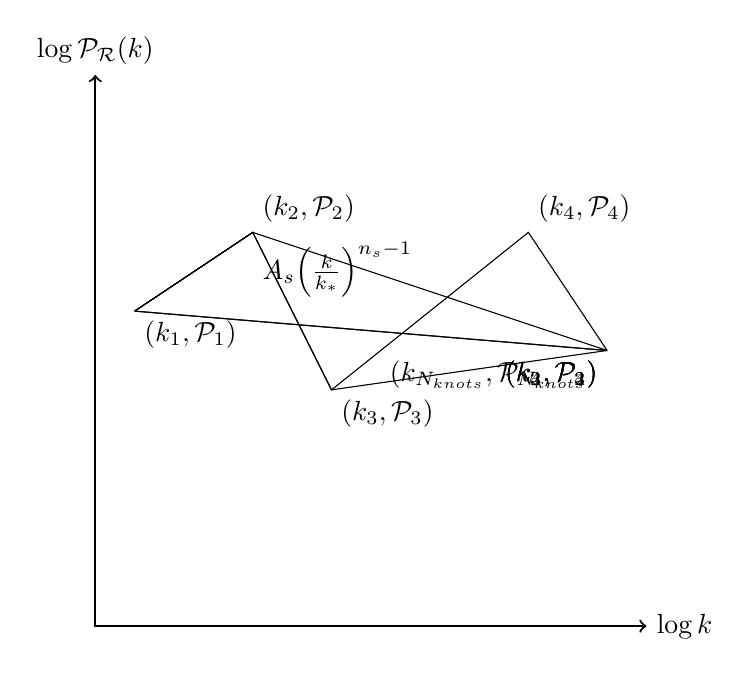
\begin{tikzpicture}
    % width of axes
      \def\xwidth{7}
      \def\ywidth{7}
    % min coordinate
      \def\xmn{0.5}
      \def\ymn{4}
    % start coordinate
      \def\xstart{2}
      \def\ystart{5}
    % middle coordinate
      \def\xmid{3}
      \def\ymid{3}
    % end coordinate
      \def\xend{5.5}
      \def\yend{5}
    % max coordinate
      \def\xmx{6.5}
      \def\ymx{3.5}

    % length of crosses
      \def\croslen{0.4}


    % Draw axes
      \draw<1-5|handout:0> [<->,thick] (0,\ywidth) node (yaxis) [above] {$\log\mathcal{P}_\mathcal{R}(k)$}
      |- (\xwidth,0) node (xaxis) [right] {$\log k$};
    % Draw limits
      %\draw [-,dashed] (\xmn,0) node[below] {$\log_{10}k_1$} -- (\xmn,\ywidth) ;
      %\draw [-,dashed] (\xmx,0) node[below] {$\log_{10}k_N$} -- (\xmx,\ywidth) ;

      \draw<1|handout:0> (\xmn,\ymn) -- (\xmx,\ymx);
      \draw<1|handout:0> (\xstart,\ystart) node[below right] {$A_s {\left(\frac{k}{k_*}\right)}^{n_s-1}$};

    % Draw the line joining start and end

      \coordinate (mn) at (\xmn,\ymn);
      \coordinate (start) at (\xstart,\ystart);
      \coordinate (mid) at (\xmid,\ymid);
      \coordinate (end) at (\xend,\yend);
      \coordinate (mx) at (\xmx,\ymx);
      \draw<2|handout:0> (mn) -- (mx);
      \draw<2-5|handout:0> (mn) node[below right]    {$(k_1,\mathcal{P}_{1})$};
      \draw<2|handout:0> (mx) node[below left]     {$(k_{2},\mathcal{P}_{{2}})$};
      \onslide<2-5|handout:0>{\movablevert{mn}};
      \onslide<2-5|handout:0>{\movablevert{mx}};

      \draw<3|handout:0> (mn) -- (start) -- (mx);
      \onslide<3-5|handout:0>{\movablecross{start}};
      \draw<3-5|handout:0> (start) node[above right] {$(k_2,\mathcal{P}_{2})$};
      \draw<3|handout:0> (mx) node[below left]     {$(k_{3},\mathcal{P}_{{3}})$};
 
      \draw<4|handout:0> (mn) -- (start) -- (mid) -- (mx);
      \onslide<4-5|handout:0>{\movablecross{mid}};
      \draw<4-5|handout:0> (mid) node[below right] {$(k_3,\mathcal{P}_{3})$};
      \draw<4|handout:0> (mx) node[below left]     {$(k_{4},\mathcal{P}_{{4}})$};

      \draw<5|handout:0> (mn) -- (start) -- (mid) -- (end) -- (mx);
      \onslide<5|handout:0>{\movablecross{end}};
      \draw<5|handout:0> (end) node[above right] {$(k_4,\mathcal{P}_{4})$};
      \draw<5|handout:0> (mx) node[below left]     {$(k_{N_\text{knots}},\mathcal{P}_{N_\text{knots}})$};


      %\draw<2-|handout:0> (\xmn,\ymn) coordinate (mn) -- (\xstart,\ystart) coordinate (start) -- (\xmid,\ymid) coordinate (mid) --  (\xend,\yend) coordinate(end) -- (\xmx,\ymx) coordinate(mx);

    % Draw the point labels
      %\draw<2-|handout:0> (mn) node[below right]    {$(k_1,\mathcal{P}_{1})$};
      %\draw<2-|handout:0> (start) node[above right] {$(k_2,\mathcal{P}_{2})$};
      %\draw<2-|handout:0> (mid) node[below right]   {$(k_3,\mathcal{P}_{3})$};
      %\draw<2-|handout:0> (end) node[above right]   {$(k_4,\mathcal{P}_{4})$};
      %\draw<2-|handout:0> (mx) node[below left]     {$(k_{N_\text{knots}},\mathcal{P}_{N_\text{knots}})$};

    % Draw a dashed line indicating the coordinate names
      %\draw[dashed] (yaxis |- start) node[left] {$y_{1}$}
      %-| (xaxis -| start) node[below] {$x_1$};
      %\draw[dashed] (yaxis |- mid) node[left] {$y_{2}$}
      %-| (xaxis -| mid) node[below] {$x_2$};
      %\draw[dashed] (yaxis |- end) node[left] {$y_{N}$}
      %-| (xaxis -| end) node[below] {$x_N$};
      %\draw  (xaxis -| start) node[below] {$\log_{10}k_2$};
      %\draw  (xaxis -| mid) node[below] {$\log_{10}k_3$};
      %\draw  (xaxis -| end) node[below] {$\log_{10}k_4$};

      % Draw the crosses
      %\onslide<2-|handout:0>{\movablevert{mn}
      %\movablecross{start}
      %\movablecross{mid}
      %\movablecross{end}
      %\movablevert{mx}
    %};

    % put some ellipses in between the start and end point

    \end{tikzpicture}

  }
  }




    \includegraphics<6|handout:0>[width=\textwidth]{figures/pps_both_1}
    \includegraphics<7|handout:0>[width=\textwidth]{figures/pps_both_2}
    \includegraphics<8|handout:0>[width=\textwidth]{figures/pps_both_3}
    \includegraphics<9|handout:0>[width=\textwidth]{figures/pps_both_4}
    \includegraphics<10|handout:0>[width=\textwidth]{figures/pps_both_5}
    \includegraphics<11|handout:0>[width=\textwidth]{figures/pps_both_6}
    \includegraphics<12|handout:0>[width=\textwidth]{figures/pps_both_7}
    \includegraphics<13|handout:0>[width=\textwidth]{figures/pps_both_8}
    \includegraphics<14|handout:0>[width=\textwidth]{figures/pps_evidence}
    \includegraphics<15          >[width=\textwidth]{figures/pps_both}
    \includegraphics<16|handout:0>[width=\textwidth]{figures/DKL.pdf}

  \end{columns}
\end{frame}

\begin{frame}
    \frametitle{REACH: Global 21cm cosmology [\href{https://www.nature.com/articles/s41550-022-01709-9}{NatAstro}]}
    \begin{columns}
        \column{0.62\textwidth}
        \begin{itemize}
            \item Imaging the universal dark ages using CMB backlight.
            \item $21\text{cm}$ hyperfine line emission from neutral hydrogen.
            \item Global experiments measure monopole across frequency.
            \item Gives a specific absorption trough, which if detected allows constraints on the physics of the dark ages decade(s) before SKA.
            \item Challenge: science hidden in foregrounds $\sim 10^4\times$signal.
        \includegraphics[height=0.3\textwidth]{figures/EDGES_antenna}
        \includegraphics[height=0.3\textwidth]{figures/SARAS}
        \includegraphics[height=0.3\textwidth]{figures/REACH_2.jpg}
        \end{itemize}

        \column{0.38\textwidth}
        \includegraphics[width=\textwidth]{figures/21cm_1.png}
        \includegraphics[width=\textwidth]{figures/21cm.png}


    \end{columns}

\end{frame}

\begin{frame}
    \frametitle{REACH: Global 21cm cosmology [\href{https://www.nature.com/articles/s41550-022-01709-9}{NatAstro}]}
    \begin{columns}
        \column{0.65\textwidth}
        \begin{itemize}
            \item EDGES~[\href{https://www.nature.com/articles/nature25792}{Nat}] claimed a controversial 2019 detection.
            \item SARAS3~[\href{https://www.nature.com/articles/s41550-022-01610-5}{NatAstro}]  would have detected this by 2021.
            \item REACH~[\href{https://www.nature.com/articles/s41550-022-01709-9}{NatAstro}] aims to settle the debate.
                \begin{itemize}
                    \item Broader band,
                    \item Honesty about systematic modelling,
                    \item State of the art inference.
                \end{itemize}
            \item Create parameterised models of sky, beam and signal, breaking degeneracy with a time-dependent likelihood to measure all three simultaneously.
            \item Use model comparison based reconstruction to determine complexity of parameterisation.
            \item Use model comparison to select likelihoods.
            \item A collaboration powered by nested sampling.
        \end{itemize}

        \column{0.35\textwidth}
        \includegraphics[width=\textwidth]{figures/EDGES}
        \begin{center}
            \includegraphics[width=0.8\textwidth]{figures/REACH_1}
        \end{center}
    \end{columns}

\end{frame}

%\begin{frame}
%    \frametitle{Nested Sampling with Likelihood Free Inference}
%    \begin{columns}
%        \column{0.5\textwidth}
%        \includegraphics[width=\textwidth]{figures/three_ways_II.pdf}
%
%        \hfill Alsing \textit{et al.}~\arxiv{1903.00007}
%    \begin{itemize}
%        \item In density estimation likelihood free inference, the output is to learn one/all of:
%            \begin{description}
%                \item[Likelihood] $P(D|\theta)$,
%                \item[Posterior] $P(\theta|D)$,
%                \item[Joint] $P(D,\theta)$.
%            \end{description}
%        \item In the first instance, nested sampling can be used to scan these learnt functions.
%    \end{itemize}
%        \column{0.5\textwidth}
%    \begin{itemize}
%        \item Data are compressed, so joint space $(D,\theta)$ is navigable by off-the-shelf codes. 
%            \begin{itemize}
%                \item Sanity checking the solution,
%                \item Computing evidences/Kullback Liebler divergences from likelihoods.
%            \end{itemize}
%        \item Its self-tuning capacity and ability to handle multi-modal distributions can be very useful for diagnosing incompletely learnt functions.
%        \item Emulated likelihoods (e.g. normalising flows) are generally fast, so can deploy more likelihood hungry techniques like NS.
%        \item In principle can use it to train emulators by marginalisation rather than maximisation.
%    \end{itemize}
%    \end{columns}
%\end{frame}
%
%\begin{frame}
%    \frametitle{Nested Sampling for Approximate Bayesian Computation/SBI}
%    \begin{columns}
%        \column{0.5\textwidth}
%        \begin{itemize}
%            \item Assume one has a generative model capable of turning parameters into mock data $D(\theta)$.
%            \item Given infinite computing power, ABC works by selecting $\{\theta : D(\theta)=D_\text{observed}\}$.
%            \item These are samples from the posterior, without using a likelihood.
%            \item In practice $D=D_\text{obs}$ becomes $D\approx D_\text{obs}$.
%            \item i.e. $|D-D_\text{obs}|<\varepsilon$, or more generally $\boxed{\rho(D,D_\text{obs})<\varepsilon}$, where $\rho$ is some suitably chosen objective function.
%            \item Main challenges are 
%                \begin{enumerate}
%                    \item Choice of $\rho$/summary stats,
%                    \item Choice of $\varepsilon$ schedule,
%                    \item Rejection sampling.
%                \end{enumerate}
%        \end{itemize}
%        \column{0.5\textwidth}
%        \begin{itemize}
%            \item Nested sampling fits this well: In principle, can just change the usual hard likelihood constraints $\{\theta\sim\pi : \mathcal{L}(\theta)>\mathcal{L}_*\}$ to
%                \[\{\theta~\sim\pi : \rho(D(\theta),D_\text{obs})<\varepsilon\}\]
%            (Brewer \& Foreman-Mackey~\arxiv{1606.03757})
%            \item Ongoing work with Andrew Fowlie \& Sebastian Hoof
%                \begin{itemize}
%                    \item How to deal with nondeterminism,
%                    \item How to interpret $\rho$ as a ``likelihood'',
%                    \item How to interpret the evidence $\mathcal{Z}$.
%                \end{itemize}
%        \end{itemize}
%    \end{columns}
%\end{frame}

%\begin{frame}
%    \frametitle{Nested sampling for truncated methods}
%
%    \begin{columns}
%        \column{0.55\textwidth}
%        \begin{itemize}
%            \item Will hear more on this tomorrow from Christoph
%            \item Many Likelihood implicit approaches at the moment have some element of sampling direct from the prior
%            \item Inefficient if number of parameters $>\mathcal{O}(\text{a few})$
%            \item Can get round this by truncating to region:
%                \[ \Gamma\{ \theta\in \text{supp} p(\theta) \:|\: p(\theta|x_0)>\bar\varepsilon\} \]
%            \item At the moment regions defined by nested boxes
%            \item \textbf{Frontier:} This seems ripe for replacement by NS -- PhD student currently working on this (Kilian Scheutwinkel)
%        \end{itemize}
%        \column{0.45\textwidth}
%        \includegraphics[width=\textwidth]{figures/tmnre}
%
%        \hfill Cole \textit{et al.}~\arxiv{2111.08030}
%    \end{columns}
%    
%\end{frame}

\begin{frame}
    \frametitle{Beyond the meta-algorithm}
    \begin{columns}
        \column{0.5\textwidth}
        \begin{itemize}
            \item Dynamic nested sampling~\arxiv{1704.03459}
            \item Unwoven nested sampling~\arxiv{1703.09701}
            \item Accelerated nested sampling~\arxiv{2212.01760}
            \item Precision nested sampling~\arxiv{2006.03371}
            \item Multiobjective nested sampling
            \item Nested sampling with gradients?
            \item Reversible nested sampling?
            \item Transdimensional nested sampling?
            \item postprocessing: \texttt{anesthetic}~\arxiv{1905.04768}
            \item crosschecking: \texttt{nestcheck}~\arxiv{1804.06406}
            \item See ``Frontiers of nested sampling'' talk from last year: \href{https://www.willhandley.co.uk/talks}{willhandley.co.uk/talks}
        \end{itemize}
        \column{0.5\textwidth}
        \includegraphics[width=\textwidth]{figures/dynesty.pdf}
        \includegraphics[width=\textwidth]{figures/supernest.pdf}
    \end{columns}
\end{frame}


\begin{frame}
    \frametitle{Conclusions}
    \begin{columns}
        \column{0.65\textwidth}
    \begin{itemize}
        \item Nested sampling is a multi-purpose numerical tool for:
            \begin{itemize}
                \item Numerical integration $\int f(x) dV$,
                \item Exploring/scanning/optimising \textit{a priori} unknown functions,
                \item Performing Bayesian inference and model comparison.
            \end{itemize}
        \item It is applied widely across cosmology and particle physics.
        \item It can be applied to both Bayesian and Frequentist inference.
    \end{itemize}
        \column{0.35\textwidth}
    \includegraphics[height=0.6\textwidth]{figures/pps_both}%
    \includegraphics[height=0.6\textwidth]{figures/REACH_2}%
    \end{columns}
    \includegraphics[height=0.2\textwidth]{figures/integration}%
    \includegraphics[height=0.2\textwidth]{figures/curvature_3}%
    \includegraphics[height=0.2\textwidth]{figures/ALP_3}%
\end{frame}


\appendix
\begin{frame}
    \frametitle{How does Nested Sampling compare to other approaches?}
    \begin{columns}
        \column{0.7\textwidth}
        \begin{itemize}
            \item In all cases:
                \begin{itemize}
                    \item[$+$] NS can handle multimodal functions
                    \item[$+$] NS computes evidences, partition functions and integrals
                    \item[$+$] NS is self-tuning/black-box
                \end{itemize}
        \end{itemize}
        \column{0.3\textwidth}
        Modern Nested Sampling algorithms can do this in $\sim\mathcal{O}(100s)$ dimensions
    \end{columns}
    \begin{columns}[t]
        \column{0.3\textwidth}
        \begin{block}{Optimisation}
            \begin{itemize}
                \item Gradient descent
                    \begin{itemize}
                        \item[$-$] NS cannot use gradients
                        \item[$+$] NS does not require gradients
                    \end{itemize}
                \item Genetic algorithms
                    \begin{itemize}
                        \item[$+$] NS discarded points have statistical meaning
                    \end{itemize}
            \end{itemize}
        \end{block}
        \column{0.3\textwidth}
        \begin{block}{Sampling}
            \begin{itemize}
                \item Metropolis-Hastings?
                    \begin{itemize}
                        \item[$-$] Nothing beats well-tuned customised MH
                        \item[$+$] NS is self tuning
                    \end{itemize}
                \item Hamiltonian Monte Carlo?
                    \begin{itemize}
                        \item[$-$] In millions of dimensions, HMC is king
                        \item[$+$] NS does not require gradients
                    \end{itemize}
            \end{itemize}
        \end{block}
        \column{0.3\textwidth}
        \begin{block}{Integration}
            \begin{itemize}
                \item Thermodynamic integration
                    \begin{itemize}
                        \item[$+$] protective against phase trasitions
                        \item[$+$] No annealing schedule tuning 
                    \end{itemize}
                \item Sequential Monte Carlo
                    \begin{itemize}
                        \item[$-$] SMC experts classify NS as a kind of SMC
                        \item[$+$] NS is athermal
                    \end{itemize}
            \end{itemize}
        \end{block}
    \end{columns}
\end{frame}

\begin{frame}
    \frametitle{Nested Sampling: a user's guide}
    \begin{enumerate}
        \item Nested sampling is a likelihood scanner, rather than posterior explorer.
            \begin{itemize}
                \item This means typically most of its time is spent on burn-in rather than posterior sampling.
                \item Changing the stopping criterion from $10^{-3}$ to $0.5$ does little to speed up the run, but can make results very unreliable.
            \end{itemize}
        \item The number of live points $n_\text{live}$ is a resolution parameter.
            \begin{itemize}
                \item Run time is linear in $n_\text{live}$, posterior and evidence accuracy goes as $\frac{1}{\sqrt{n_\text{live}}}$.
                \item Set low for exploratory runs $\sim\mathcal{O}(10)$ and increased to $\sim\mathcal{O}(1000)$ for production standard.
            \end{itemize}
        \item Most algorithms come with additional reliability parameter(s).
            \begin{itemize}
                \item e.g. \texttt{MultiNest}: $\texttt{eff}$, \texttt{PolyChord}: $n_\text{repeats}$.
                \item These are parameters which have no gain if set too conservatively, but increase the reliability.
                \item Check that results do not degrade if you reduce them from defaults, otherwise increase.
            \end{itemize}
    \end{enumerate}
\end{frame}




\begin{frame}
    \frametitle{Occam's Razor~\arxiv{2102.11511}}
    \begin{itemize}
        \item Bayesian inference quantifies Occam's Razor:
            \begin{itemize}
                \item \textit{``Entities are not to be multiplied without necessity''} \hfill --- William of Occam
                \item \textit{``Everything should be kept as simple as possible, but not simpler''} \hfill --- ``Albert Einstein''
            \end{itemize}
        %\item Consider the Evidence $\C[3]{\mathcal{Z}\equiv P(D|M)}$: 
        %    \begin{description}[Parameter estimation]
        %        \item [Parameter estimation] normalisation constant
        %        \item [Model comparison] critical update factor for \C[5]{model prior} to \C[4]{model posterior}
        %    \end{description}
        \item Properties of the evidence: rearrange Bayes' theorem for parameter estimation
            \[\C[0]{\mathcal{P}(\theta)} = \frac{\C[2]{\mathcal{L}(\theta)} \C[1]{\pi(\theta)}}{\C[3]{\mathcal{Z}}} \qquad\Rightarrow\qquad \C[3]{\log \mathcal{Z}} = \C[2]{\log\mathcal{L}(\theta)} - \log \frac{\C[0]{\mathcal{P}(\theta)}}{\C[1]{\pi(\theta)}}.\]  
        \item Evidence is composed of a ``goodness of fit'' term  and ``Occam Penalty''.
    \end{itemize}
    \begin{columns}[t]
        \column{0.5\textwidth}
    \begin{itemize}
        \item RHS true for all $\theta$. Take max likelihood value $\theta_*$:
            \[
                \log \mathcal{Z} = -\chi_\text{min}^2 - \text{Mackay penalty.}
            \]
    \end{itemize}
        \column{0.5\textwidth}
    \begin{itemize}
        \item Be more Bayesian and take posterior average to get the ``Occam's razor equation''
            \[
                \boxed{
                    \log \mathcal{Z} = \av[\mathcal{P}]{\log\mathcal{L}} - \mathcal{D}_\text{KL}.
            }
            \]
    \end{itemize}
    \end{columns}
    \vfill
    \begin{itemize}
        \item Natural regularisation which penalises models with too many parameters.
    \end{itemize}
\end{frame}

\begin{frame}
    \frametitle{Kullback Liebler divergence}
    \begin{columns}
        \column{0.5\textwidth}
        \begin{itemize}
            \item The KL divergence between \C[1]{prior $\pi$} and \C[0]{posterior $\mathcal{P}$} is is defined as:
                \[\mathcal{D}_\text{KL} = \av[\mathcal{P}]{\log\frac{\mathcal{P}}{\pi}} = \int \mathcal{P}(\theta) \log \frac{\mathcal{P}(\theta)}{\pi(\theta)}d\theta.\]
            \item Whilst not a distance, $\mathcal{D}=0$ when $\mathcal{P}=\pi$.
            \item Occurs in the context of machine learning as an objective function for training functions.
            \item In Bayesian inference it can be understood as a log-ratio of ``volumes'':
                \[ \mathcal{D}_\text{KL} \approx \log \frac{V_\pi}{V_\text{P}}.\]
                (this is exact for top-hat distributions).
        \end{itemize}
        \column{0.5\textwidth}
        \includegraphics{figures/volumes.pdf}
    \end{columns}
\end{frame}

\begin{frame}
    \frametitle{Statistics: fast estimation of small $p$-values~\arxiv{2106.02056}(PRL)}
    \begin{columns}
        \column{0.55\textwidth}
        \begin{itemize}
            \item Nested sampling for frequentist computation!?
            \item $p$-value: $P(\lambda>\lambda^*|H_0)$ -- probability that test statistic $\lambda$ is at least as great as observed $\lambda^*$.
            \item Computation of a tail probability from sampling distribution of $\lambda$ under $H_0$.
            \item For gold-standard $5\sigma$, this is very expensive to simulate directly ($\sim10^9$ by definition).
            \item Need insight/approximation to make efficient.
            \item Nested sampling is tailor-made for this, just make switch: $X\leftrightarrow p$, $\mathcal{L}\leftrightarrow\lambda$, $\theta \leftrightarrow x$.
            \item The only real conceptual shift is switching the integrator from parameter- to data-space.
        \end{itemize}
        \column{0.45\textwidth}
        \includegraphics[width=\textwidth]{figures/pvalue.pdf}
    \end{columns}
    
\end{frame}

\begin{frame}
    \frametitle{Exploration of phase space~\arxiv{2106.02056}}
    \begin{columns}
        \column{0.5\textwidth}
        \begin{itemize}
            \item Nested sampling for cross section computation/event generation.
            \item Numerically compute collisional cross section 
                \vspace{-5pt}\[\sigma = \int_\Omega d\Phi |\mathcal{M}|^2,\]
                $\Omega$ phase space of kinematic configurations $\Phi$, each with matrix element $\mathcal{M}(\Phi)$.
            \item Current state of the art e.g. HAAG (improvement on RAMBO) requires knowledge of $\mathcal{M}(\Phi)$.
            \item Nested sampling can explore the phase space and compute integral blind with comparable efficiency.
        \end{itemize}
        \column{0.5\textwidth}
        \includegraphics[width=\textwidth]{figures/phase_space_1.pdf}
        \includegraphics[width=\textwidth]{figures/phase_space.pdf}
    \end{columns}
\end{frame}

\begin{frame}
    \frametitle{Quantification of fine tuning~\arxiv{2101.00428}~\arxiv{2205.13549}}
    \vspace{-10pt}
    \begin{columns}
        \column{0.55\textwidth}
        \begin{itemize}
            \item Example: Cosmological constraints on decaying axion-like particles~\arxiv{2205.13549}.
            \item Subset of parameters $\xi,m_a,\tau,g_{a\gamma}$: ALP fraction, mass, lifetime and photon coupling.
                {(\small Also vary cosmology, $\tau_n$ and nuisance params)}
            \item Data: CMB, BBN, FIRAS, SMM, BAO.
            \item Standard profile likelihood fit shows ruled out regions and best-fit point.
            \item<2-> Nested sampling scan:
                \begin{itemize}
                    \item Quantifies amount of parameter space ruled out with Kullback-Liebler divergence $\mathcal{D}_\mathrm{KL}$.
                    \item Identifies best fit region as statistically irrelevant from information theory/Bayesian.
                    \item No evidence for decaying ALPs. Fit the data equally well: but more constrained parameters create Occam penalty.
                \end{itemize}
        \end{itemize}
        \column{0.45\textwidth}
        \includegraphics<1|handout:0>[width=\textwidth]{figures/ALP_1.pdf}
        \includegraphics<2          >[width=\textwidth]{figures/ALP_2.pdf}
        \includegraphics<3|handout:0>[width=\textwidth]{figures/ALP_3.pdf}
    \end{columns}
    
\end{frame}




\end{document}
